\subsection{Population Generation}

\begin{table}[H]
  \centering
  \begin{tabular}{lllll}
    \textbf{Input}                           &               & \textbf{Function}            &               & \textbf{Output}         \\
    \midrule
    \textit{Terrain, PopulationAmplifier[]}      & $\rightarrow$ & \textbf{PopulationGenerator}      & $\rightarrow$ & \textit{PopulationMap}        \\
    \bottomrule
  \end{tabular}

  \caption{Definition of the PopulationGenerator function which is responsible for generating intensity map based on the terrain.}
  \label{table:popgen}
\end{table}
\vspace{-0.4cm} % Mimic spacing below figures

% Short description
The population generator populates the terrain provided as input.
Specifically, a intensity map will be generated based on the terrain, which will represent the population density for the entire terrain.
Areas of high-density population can be altered with user input, which is given as a visual option during the road generation phase.
When placed, the population density of that area will be drastically increased.
This marker placement can be repeated multiple times to generate several cities.

PopulationGenerator is responsible for creating a procedurally generated intensity map describing the population in the world.
The terrain parameter is required to generate an intensity map since it needs to mask off certain areas in the landscape, such as oceans, rivers, or mountains.
Then, the generator would use a few layers of simplex noise to create a representation of populations throughout the world.
Population markers are used to increase population density in a certain area, and these are applied after generating the initial population map.
Markers are stored within the PopulationAmplifier set, which is the second input for the PopulationGenerator.
This is useful to make sure the created cities have a higher density, but it will still respect the original population map to some degree.

\begin{figure}[h!]
  \centering
  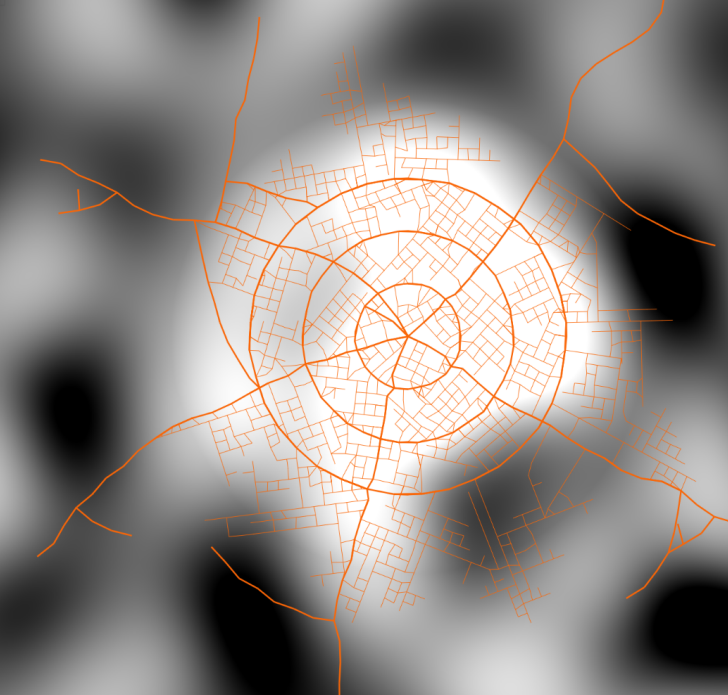
\includegraphics[width=0.5\textwidth]{figure/pop_density.png}
  \caption{An example of a population map with a Paris city generated within it.}
  \label{fig:pop_dens}
\end{figure}